\documentclass[../../main.tex]{subfiles}


\begin{document}

\subsection*{(a)}
There are 4982 Applications with an average throughput time of 21.904 as determined using the following Process:\\
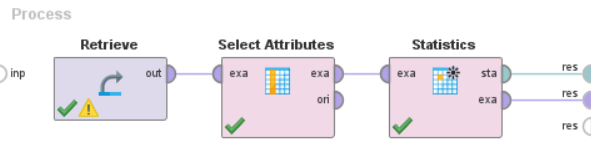
\includegraphics[width=\textwidth]{img/QUESTION_5a_PROCESS_average_throughput_time.png}

Using Celonis Process AI on our Dataset we learn that the most frequent variant (happy path) happens 320 times. This variant can be seen below.\\
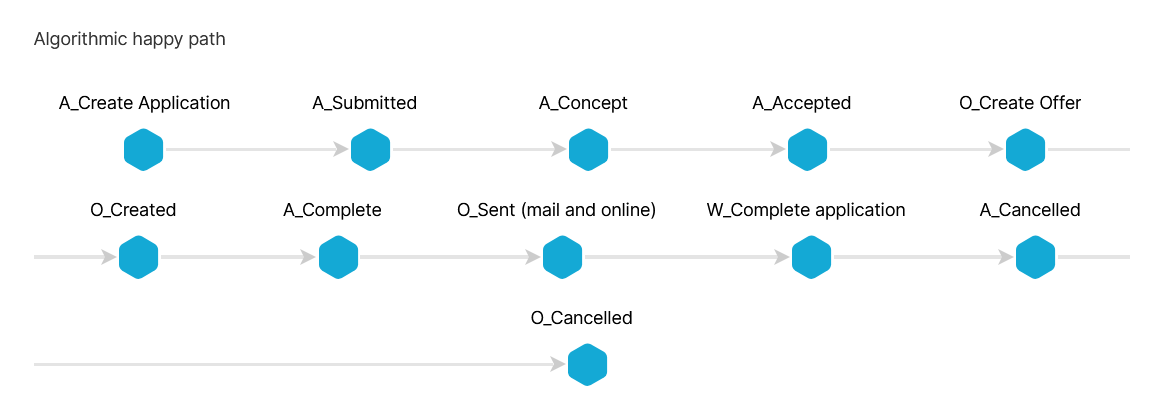
\includegraphics[width=\textwidth]{img/QUESTION_5a_happy_path.png}

The following graph shows the frequency distribution of the throughput times. As one can see they are initially quite high and eventually deteriorate in frequency until the 29-33 Day, where they spike again and after that deteriorate quickly again. The reason for the spike at 29-33 Days is probably that a new month begins/ends at this time. Therefore, many applications will likely be terminated at this time for administrative reasons.\\
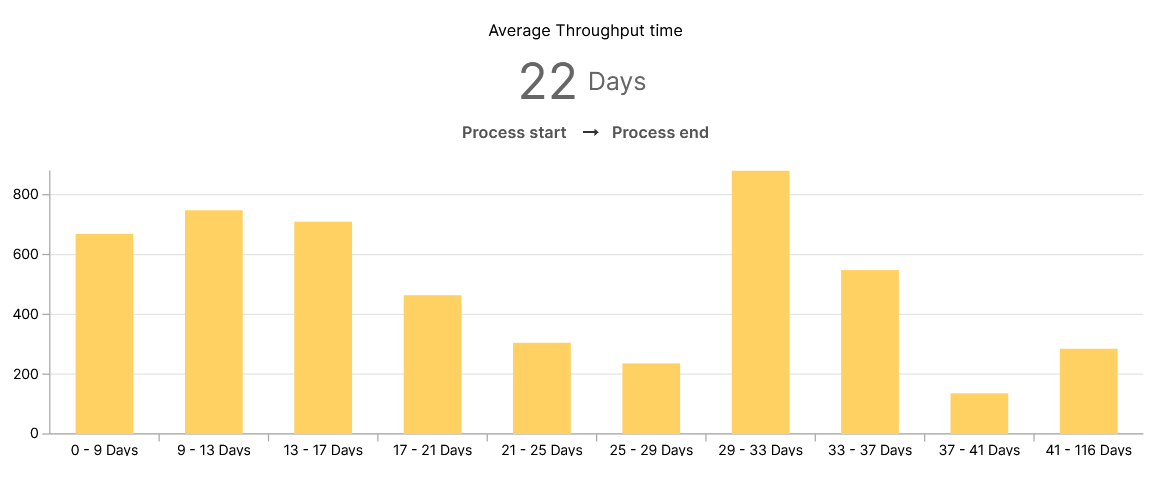
\includegraphics[width=\textwidth]{img/QUESTION_5a_throughput_time_distribution.png}


\subsection*{(b)}
% First item
The BPMN model for cases running under 30 days can be seen below (zoom in to inspect in detail). We created it by starting a new Analysis and opening a new \textit{conformance} sheet. Then we clicked \textit{Mine process model} and in the next window added a new selection for Throughput time under 30. Then we clicked \textit{select all} and \textit{Launch analysis}. We then clicked \textit{View process model} where the model below was displayed and downloadable.\\
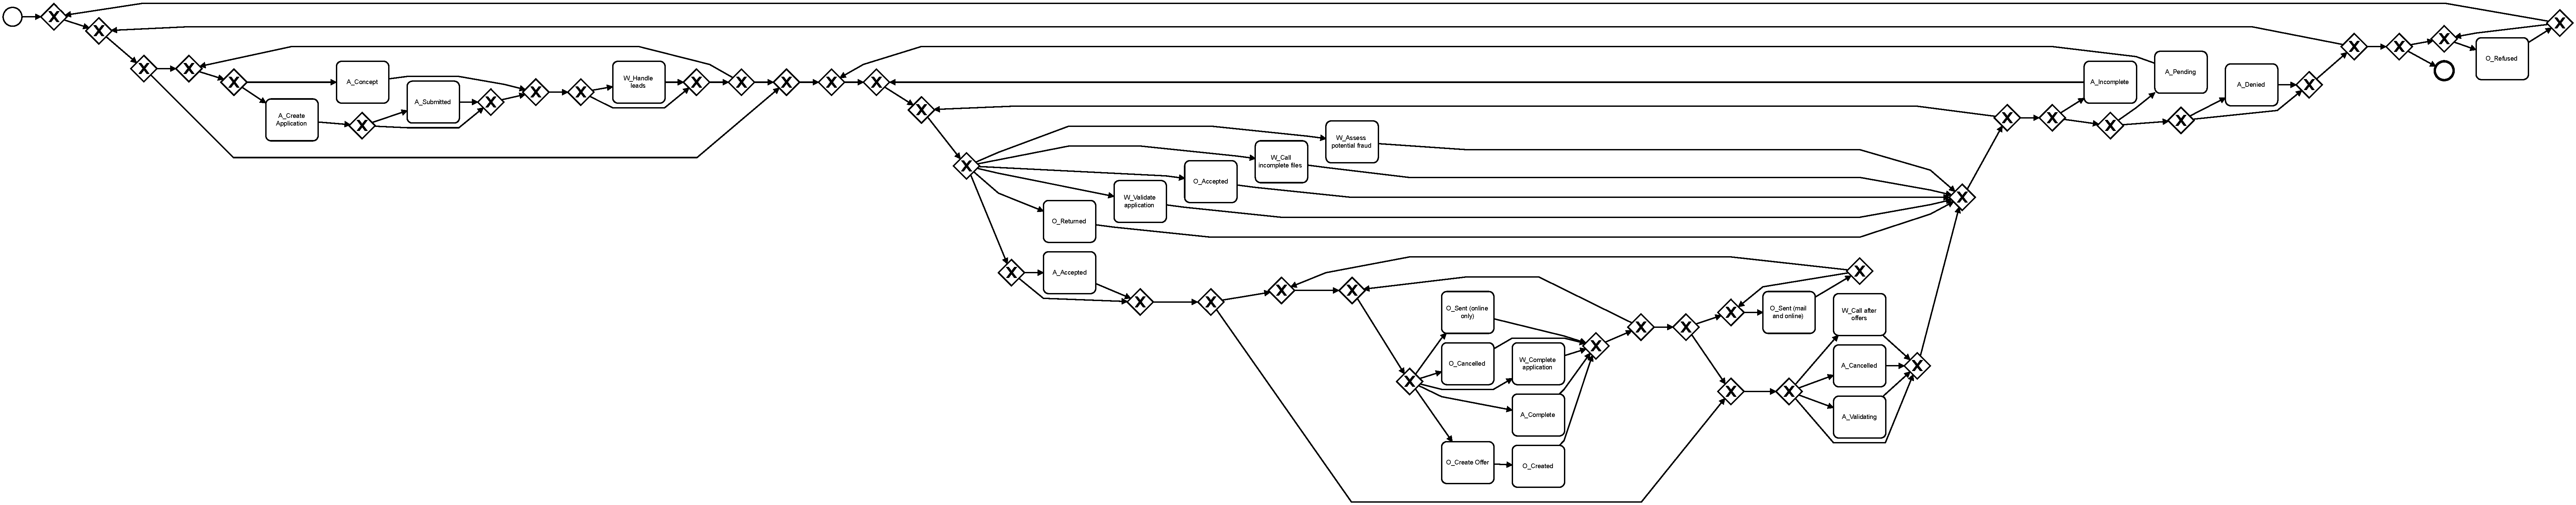
\includegraphics[width=\textwidth]{img/QUESTION_5b_BPMN_model.pdf}

% Second item
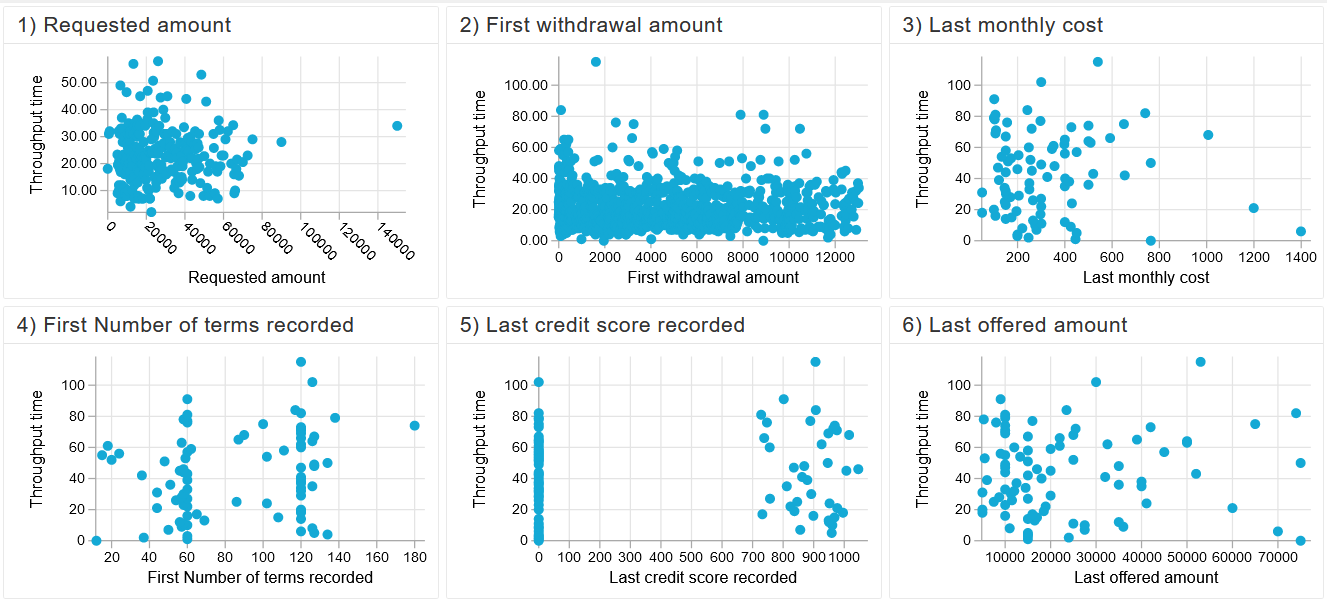
\includegraphics[width=\textwidth]{img/QUESTION_5b_scatter_plots.png}

% Third item
The DFG below was created by opening a new process explorer and only selecting the following activities to display: A$\_$Create $\_$Application, O$\_$Created, W$\_$Complete$\_$Application, O$\_$Accepted, O$\_$Refused, O$\_$Cancelled and A$\_$Cancelled. 100\% of activities and connections are being displayed. To see which edges are especially long-lasting we selected throughput time as our edge label.\\
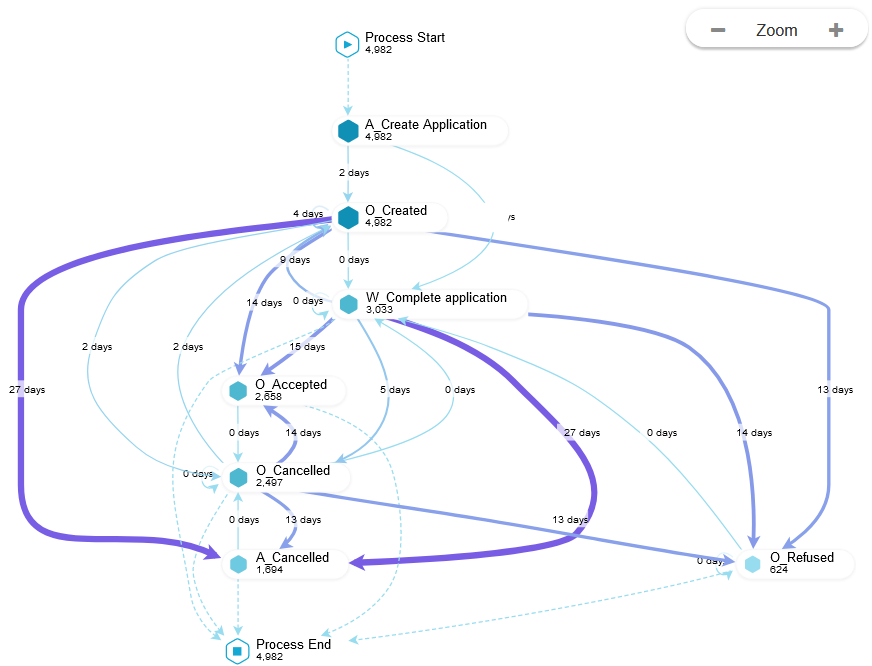
\includegraphics[width=\textwidth]{img/QUESTION_5b_DFG.png}
This way we can see that there are two very long-lasting edges (\texttt{O$\_$Created$\rightarrow$A$\_$Cancelled} and \texttt{W$\_$Complete$\_$application$\rightarrow$A$\_$Cancelled}) with a throughput time of 27 days. There is also a number of medium long-lasting edges with throughput times of 13-15 days

% Fourth item
The DFG below was created by opening a new process explorer and only selecting the following activities to display: A$\_$Create $\_$Application, O$\_$Created, W$\_$Complete$\_$Application, O$\_$Accepted, O$\_$Refused, O$\_$Cancelled and A$\_$Cancelled. 100\% of activities and connections are being displayed. We also filtered the dataset to only select cases with a throughput over 29 days.
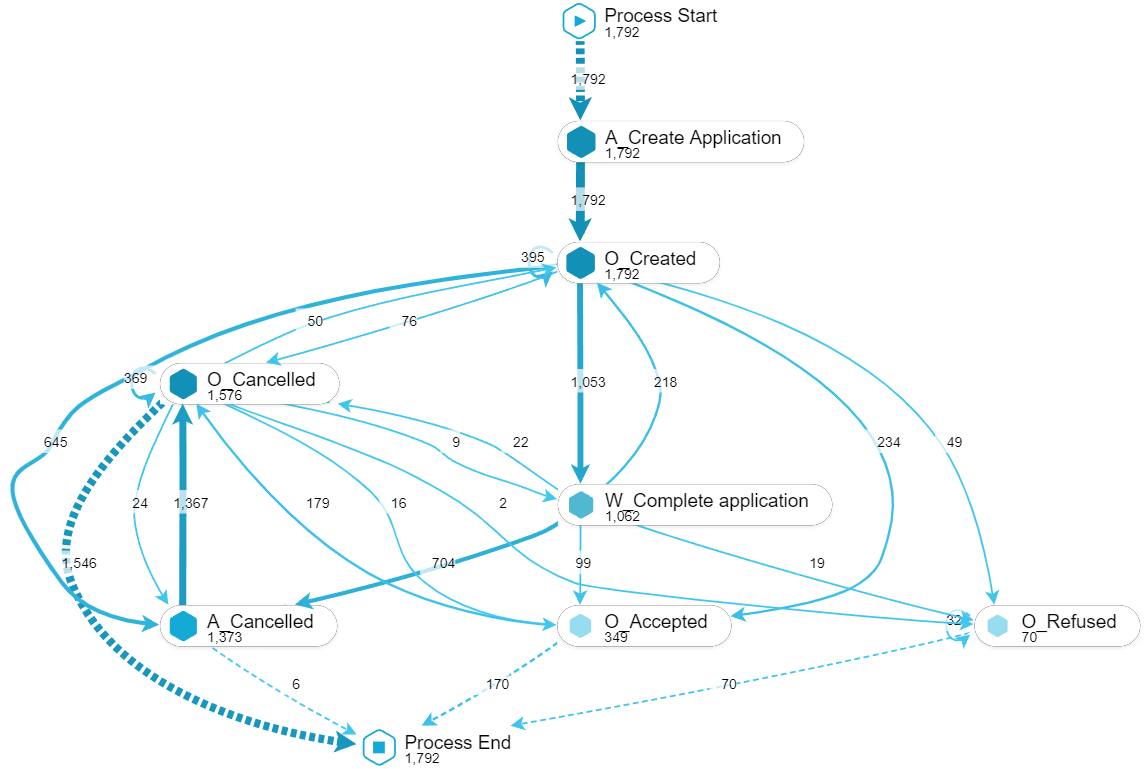
\includegraphics[width=\textwidth]{img/QUESTION_5b_over30.png}
Here we can see, that most cases with a throughput time over 29 days were cancelled. Additionally, most were passed through A$\_$Cancelled first, before passing through O$\_$Cancelled to the Process End.


\subsection*{(c)}
% first item
We select only long-lasting cases (throughput time $>$29 days) which are never cancelled:

\includegraphics[width=\textwidth]{img/QUESTION_5c_selection.png}

Of these 416 cases, the average throughput time was 40 days. The following graph shows the frequency distribution of the throughput times. As one can see, the probability to have a case, which is not cancelled, falls roughly exponentially with increase in throughput time.\\
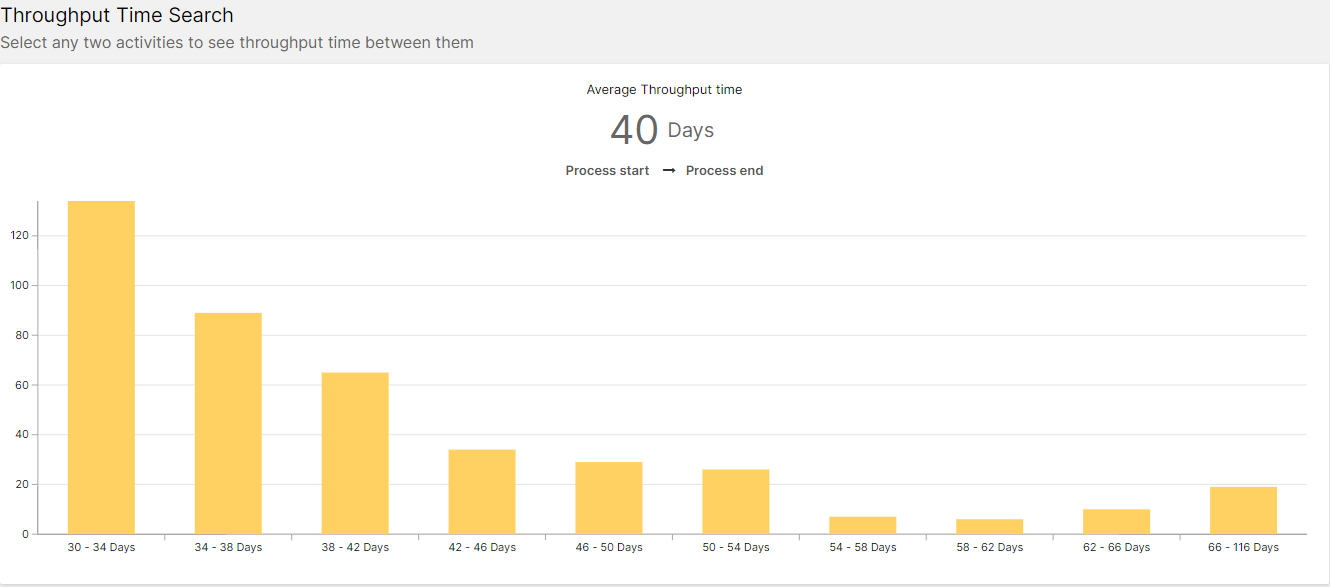
\includegraphics[width=\textwidth]{img/QUESTION_5c_throughput_time.png}

Using Celonis Process AI on our Dataset we learn that the most frequent variant (happy path) happens 7 times. This variant can be seen below.\\
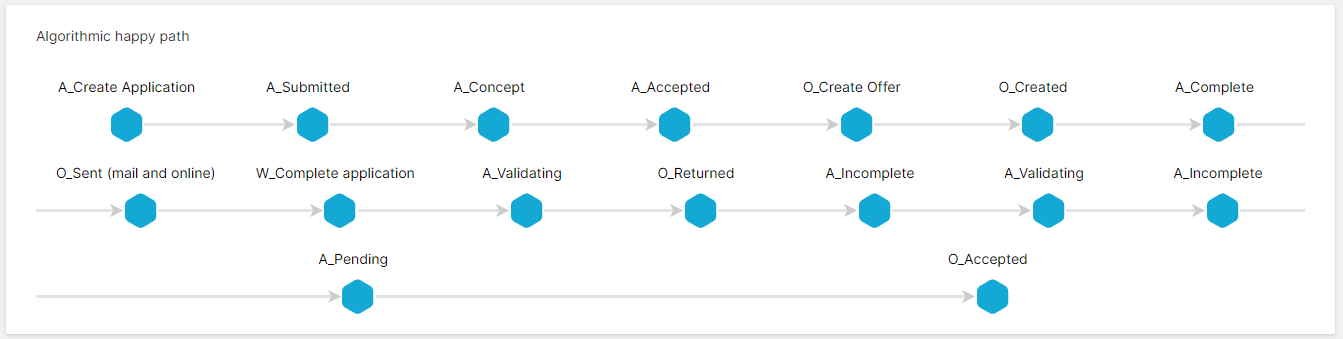
\includegraphics[width=\textwidth]{img/QUESTION_5c_happy_path.png}

% second item
Our first observation is that 37\% of the long-running cases (throughput time $>$29 days) which are never cancelled pass from W$\_$Complete$\_$Application to A$\_$Validating. We can see, that this transition by itself already takes an average of 15 days, which clearly is a big bottleneck in the whole process:\\
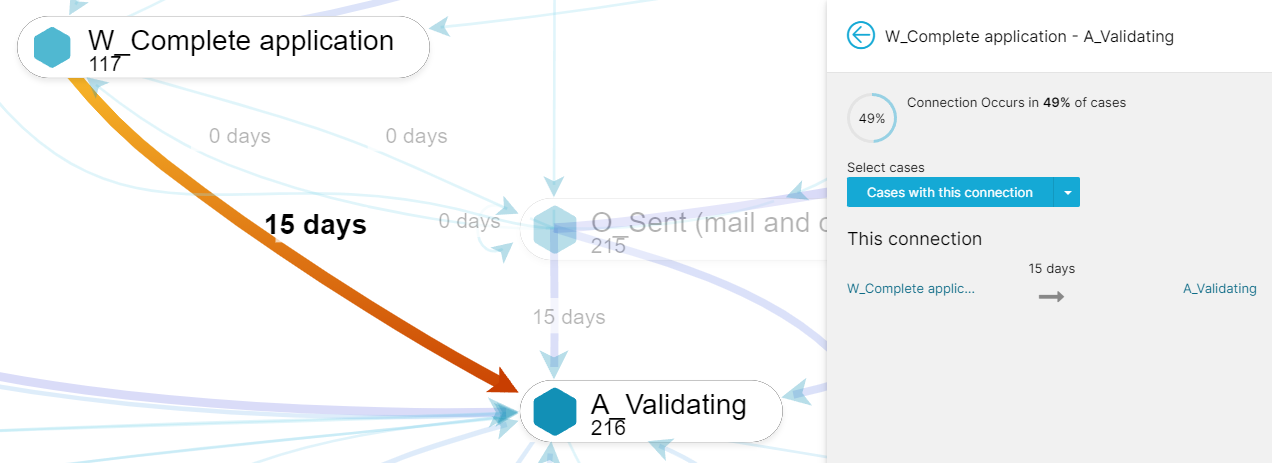
\includegraphics[width=\textwidth]{img/QUESTION_5c_W_Complete.png}

We also observed that the workflow of validating applications (W$\_$Validate$\_$Applicataion) takes 27 days on average, when it ends up being denied (in A$\_$Denied). Although not many cases pass through this transition, it seems like a huge waste of time, considering that the applications get refused (in O$\_$Refused), and the bank won't be profiting from these applicants:\\
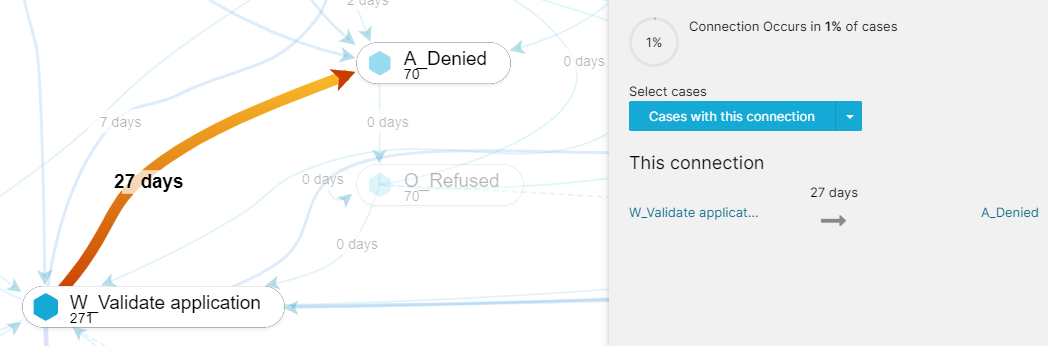
\includegraphics[width=\textwidth]{img/QUESTION_5c_W_Validate.png}

% third item
We use: \\
	\texttt{CALC$\_$THROUGHPUT(ALL$\_$OCCURRENCE['Process Start'] TO ALL$\_$OCCURRENCE['Process End'], REMAP$\_$TIMESTAMPS("Activity$\_$Table$\_$csv"."COMPLETE TIMESTAMP", DAYS))}\\
to calculate the throughput time and:\\
	\texttt{COUNT(CASE WHEN "Activity$\_$Table$\_$csv"."ACTIVITY"='O$\_$Create Offer' THEN \\ "Activity$\_$Table$\_$csv"."ACTIVITY" END )}\\
to calculate the number of offers for each case.\\
We can plot the throughput time and the number of offers on a case basis in the following scatter plot:\\
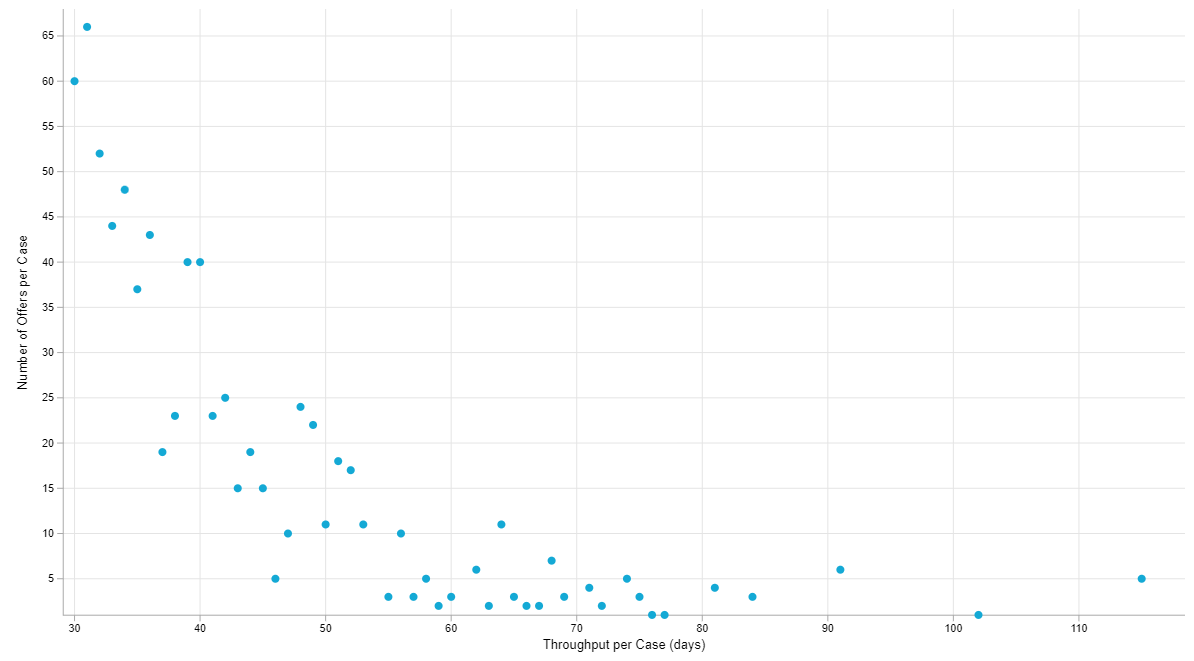
\includegraphics[width=\textwidth]{img/QUESTION_5c_scatter.png}


\subsection*{(d)}
We observed that cases over a months time in progress and still were completed were becoming less likely with increase in throughput time. We also observed for long-running cases that with increase in throughput time the number of offers per case exponentially decreased.

In question 5 c) we have detected meaningful bottlenecks in the application process. A straight forward approach to reduce average throughput time is to focus on optimizing these specific parts of the whole process. We would recommend focussing especially on the bottleneck from W$\_$Complete$\_$Application to A$\_$Validating, which 37\% of cases pass through. Herein, the most potential for gain for the bank lays.


\end{document}